% CUSTOM PACKAGES
% =================
\usepackage[shadow]{todonotes}	% \todo{}: side notes at the margins; \todo[inline]{}: inline notes; \missingfigure{}; \listoftodos
\usepackage{color, soul}	% Highlighting, use \hl{...}
\usepackage{wrapfig}	% wrap text around figures; https://en.wikibooks.org/wiki/LaTeX/Floats,_Figures_and_Captions
\usepackage{verbatim}	% comment out chunks of text
\usepackage[normalem]{ulem} % fancy underlining, strikethrough spanning pages. \sout strikethrough, \xout, \underline



% Aliases and new definitions
% =============================

\newcommand{\vdag}{(v)^\dagger}
\newcommand\aastex{AAS\TeX}
\newcommand\latex{La\TeX}

% Symbol: Approximately proportional to (http://tex.stackexchange.com/questions/33538/how-to-get-an-approximately-proportional-to-symbol)
\def\apropto{%
  \def\p{%
    \setbox0=\vbox{\hbox{$\propto$}}%
    \ht0=0.6ex \box0 }%
  \def\s{%
    \vbox{\hbox{$\sim$}}%
  }%
  \mathrel{\raisebox{0.7ex}{%
      \mbox{$\underset{\s}{\p}$}%
    }}%
}

\newcommand{\fermi}{\emph{Fermi}}

\newcommand{\nemmen}{{\bf NEMMEN, R. S.}}

\newcommand{\lat}{\emph{Fermi} LAT Collaboration}

\newcommand{\continue}{\todo[inline,color=RedOrange]{
\centerline{ \textbf{\Large CONTINUE} }   
} }

\newcommand{\mario}{
\begin{wrapfigure}{l}{0.03\textwidth}
\vspace{-20pt}
\begin{center}

\includegraphics[width=0.07\textwidth]{figures/Mario.png}
\end{center}
\vspace{-10pt}
\end{wrapfigure}
}

\newcommand{\bowser}{
\begin{wrapfigure}{l}{0.03\textwidth}
\vspace{-20pt}
\begin{center}
\reflectbox{
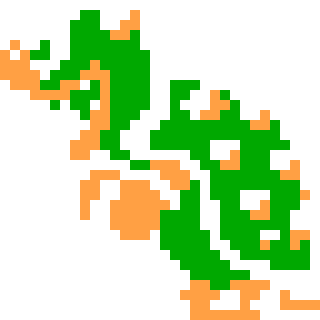
\includegraphics[width=0.07\textwidth]{figures/Bowser.png}
}
\end{center}
\vspace{-10pt}
\end{wrapfigure}
}

% Environment for pretty box with title. Colors inspired
% on default style used in http://www.lasca.ic.unicamp.br/pub/ctan/macros/latex/contrib/tcolorbox/tcolorbox.pdf
% Usage: 
% \begin{boxed}{Box title}
% This is the text formatted by the boxed environment
% \end{boxed}
\definecolor{boxback}{HTML}{DAE5F0}
\definecolor{boxframe}{HTML}{0F365B}
\newenvironment{boxnamed}[1]
{   
\begin{tcolorbox}[enhanced, drop shadow, colframe=boxframe, colback=boxback,title=#1]
}
%text goes here
{
\end{tcolorbox}   
}

% Footnote without marker, cf. http://tex.stackexchange.com/questions/30720/footnote-without-a-marker
\newcommand\orphanfoot[1]{
  \begingroup
  \renewcommand\thefootnote{}\footnote{#1}
  \addtocounter{footnote}{-1}
  \endgroup
}

% figshare
\newcommand{\figshare}{fig\textbf{share}}

% cross (wrong) symbol, needs pifont package
\newcommand{\xmark}{\ding{56}}

% OK symbol (check), needs pifont package
\newcommand{\ok}{\ding{52}}

% Useful for citations with e.g.
\newcommand{\eg}[1]{(e.g. \citealt{#1})}

% fonts for code sample: \code{text sample}
\def\code#1{\texttt{#1}}

% Sgr A*
\newcommand{\sgra}{Sgr A$^*$}

\newcommand{\per}{NGC 1275}

% red underline
\def\redul#1{{\color{red} \underline{\color{black}#1}}}




